\documentclass{beamer}
\usepackage{chronosys}
\usepackage{tikz}

\usepackage{ifpdf}
\ifpdf
\usepackage{hyperref}
%\pdfadjustspacing=1
%\fi

\mode<presentation>
 {
  \usetheme{Frankfurt}
   \usecolortheme[rgb={0.36,0.54,0.66}]{structure}
   
   \definecolor{inaf}{HTML}{1D71B8}
   %\definecolor{ashgrey}{rgb}{0.7, 0.75, 0.71}
   \definecolor{autumn}{rgb}{0.7, 0.75, 0.71}
   \definecolor{autumn1}{rgb}{0.7, 0.75, 0.71}
   \definecolor{autumn2}{rgb}{0.36, 0.54, 0.66}
   
   \definecolor{blue}{HTML}{84CECC}
   \definecolor{gr}{HTML}{375D81}

\setbeamercolor{alerted text}{fg=inaf!80!yellow}
\setbeamercolor*{palette primary}{fg=inaf!60!black,bg=autumn}
\setbeamercolor*{palette secondary}{fg=white!70!black,bg=autumn2}
\setbeamercolor*{palette tertiary}{bg=white!80!black,fg=autumn2}
\setbeamercolor*{palette quaternary}{fg=white,bg=autumn2}

\setbeamercolor*{sidebar}{fg=inaf,bg=autumn}

\setbeamercolor*{palette sidebar primary}{fg=inaf!10!black}
\setbeamercolor*{palette sidebar secondary}{fg=white}
\setbeamercolor*{palette sidebar tertiary}{fg=inaf!50!black}
\setbeamercolor*{palette sidebar quaternary}{fg=yellow!10!orange}

\setbeamercolor*{titlelike}{parent=palette primary}
\setbeamercolor{frametitle}{bg=autumn1}
\setbeamercolor{frametitle right}{bg=autumn}

\setbeamercolor*{separation line}{}
\setbeamercolor*{fine separation line}{}

\mode
<all>
   
   %\usecolortheme{wolverine}
   \usecolortheme{rose}
   \usefonttheme{serif}
%   \setbeamercolor{section in toc}{fg=red}
 }

\title[Feynman]{Vincere un Nobel per la fisica con i disegni}
\author[G.Filippelli]{Gianluigi Filippelli}
\date{Liceo "C. Cavalleri", Parabiago (Milano). 09/02/2018}

\usepackage[latin1]{inputenc}
\usepackage[italian]{babel}
\usepackage{times}
%
\begin{document}
%
\begin{frame}
 \titlepage
\end{frame}
%
% Introduzione
%
\section{Introduzione}
%
\begin{frame}[feynmanquote]
	\frametitle{Richard Feynman}
	\begin{center}
		\begin{tikzpicture}[every node/.style={inner sep=0,outer sep=0}]
			\onslide<1>\node at (0,0) () {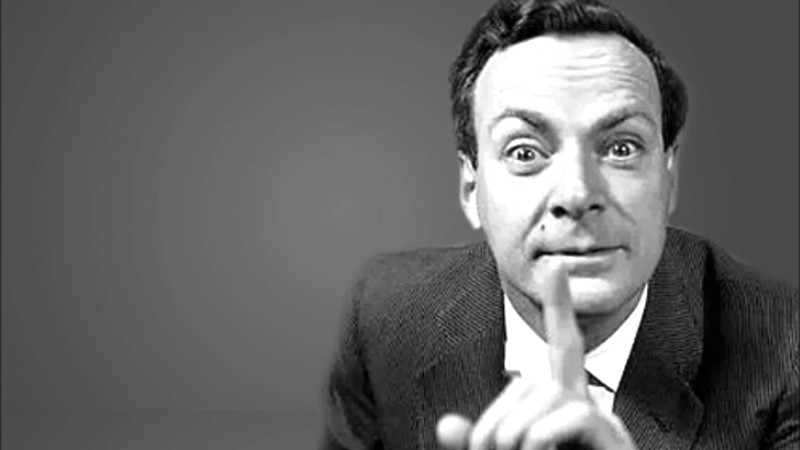
\includegraphics[width=10cm]{files/feynman.jpg}};
			\onslide<2>\node at (0,0) () {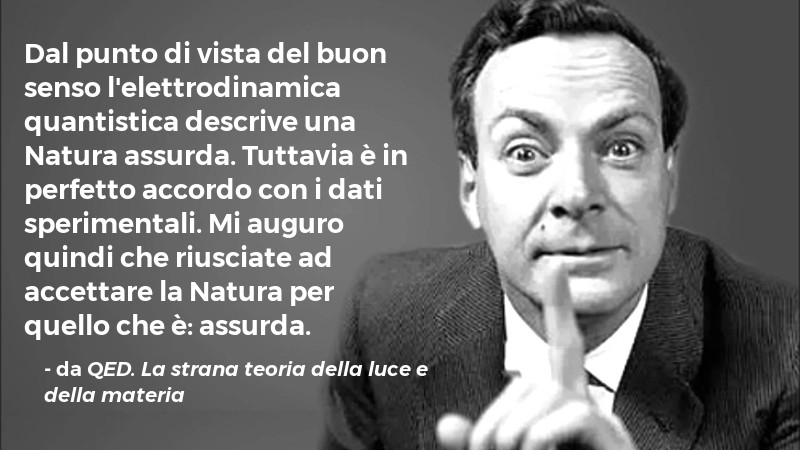
\includegraphics[width=10cm]{files/feynmanqed.jpg}};
		\end{tikzpicture}
	\end{center}
\end{frame}
%
% Modello standard
%
\section{Il modello standard}
%
\begin{frame}[standard01]
	\frametitle{La famiglia delle particelle elementari}
	\begin{center}
		{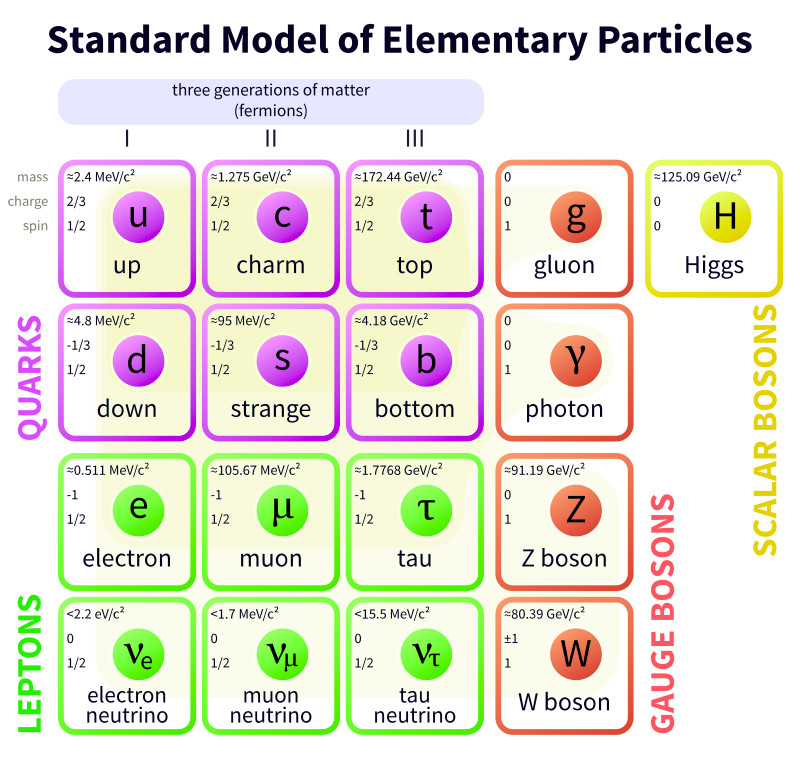
\includegraphics[width=7cm]{files/standard_model.jpg}}
	\end{center}
\end{frame}
%
\begin{frame}[interazioni01]
	\frametitle{Le interazioni fondamentali}
	\begin{enumerate}
		\item Interazione forte \onslide<2->{- $10^{38}$} \onslide<3->{- $10^{-15} m$}
		\item Interazione elettromagnetica \onslide<2->{- $10^{36}$} \onslide<3->{- $\infty$}
		\item Interazione debole \onslide<2->{- $10^{25}$} \onslide<3->{- $10^{-18} m$}
		\item Interazione gravitazionale \onslide<2->{- $1$} \onslide<3->{- $\infty$}
	\end{enumerate}
\end{frame}
%
\begin{frame}[interazioni02]
	\frametitle{Le interazioni fondamentali}
	\begin{enumerate}
		\item Interazione forte - quark, gluoni (adroni) \onslide<2->{- carica di colore}
		\item Interazione elettromagnetica - particelle cariche \onslide<2->{- carica elettrica}
		\item Interazione debole - leptoni, bosoni di gauge \onslide<2->{- carica di sapore}
		\item Interazione gravitazionale - particelle massive
		\onslide<3>{
			\begin{itemize}
				\item Deformazione geometrica dello spaziotempo dovuta alla presenza della massa
			\end{itemize}}
	\end{enumerate}
\end{frame}
%
% Diagrammi di Feynman
%
\section{I diagrammi di Feynman}
%
\subsection{Le origini}
%
\begin{frame}[cammini]
	\frametitle{I cammini di Feynman}
	\begin{center}
		\begin{tikzpicture}[every node/.style={inner sep=0,outer sep=0}]
		\onslide<1>\node at (0,0) () {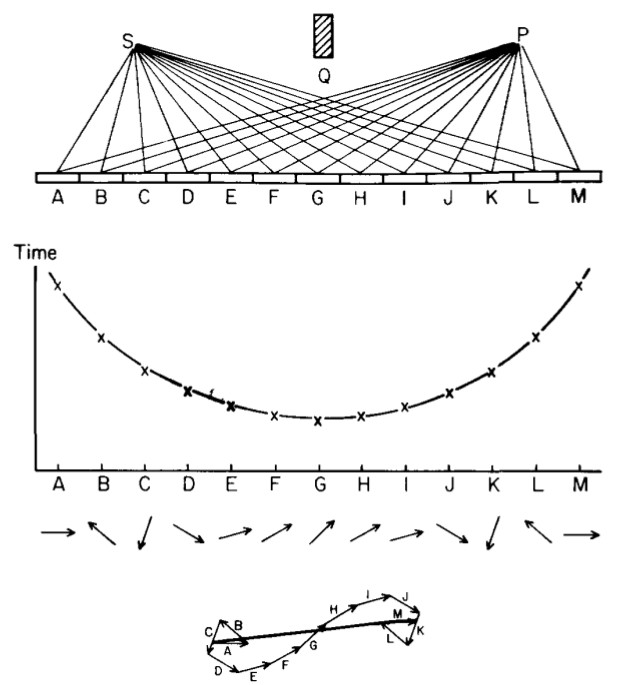
\includegraphics[width=5cm]{files/feynman_cammini.jpg}};
		\onslide<2>\node at (0,0) () {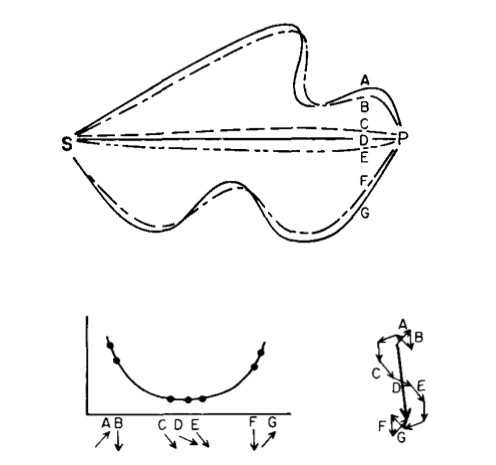
\includegraphics[width=5cm]{files/feynman_cammini02.jpg}};
		\end{tikzpicture}
	\end{center}
\end{frame}
%
\subsection{Una gustosa anteprima}
\begin{frame}[gamov]
	\frametitle{Disegnare le interazioni tra particelle}
	\begin{center}
		{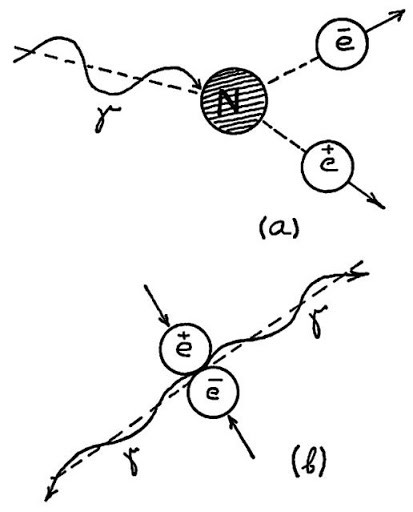
\includegraphics[width=6cm]{files/gamov.jpg}}
	\end{center}
\end{frame}
%
\subsection{Disegnare le interazioni}
\begin{frame}[diagrammi]
	\frametitle{I primi diagrammi}
	\begin{center}
		\begin{tikzpicture}[every node/.style={inner sep=0,outer sep=0}]
			\onslide<1>\node at (0,0) () {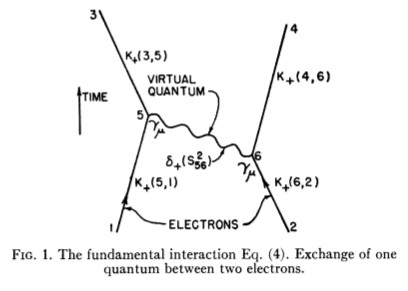
\includegraphics[width=5cm]{files/feynman_diagramma.jpg}};
			\onslide<2>\node at (0,0) () {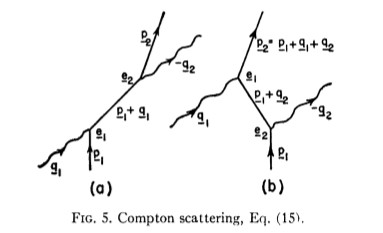
\includegraphics[width=5cm]{files/feynman_compton.jpg}};
		\end{tikzpicture}
	\end{center}
\end{frame}
%
\subsection{Feynman a scuola}
\begin{frame}[scuola01]
	\frametitle{Scambiare particelle}
	\begin{center}
		\begin{tikzpicture}[every node/.style={inner sep=0,outer sep=0}]
			\onslide<1>\node at (0,0) () {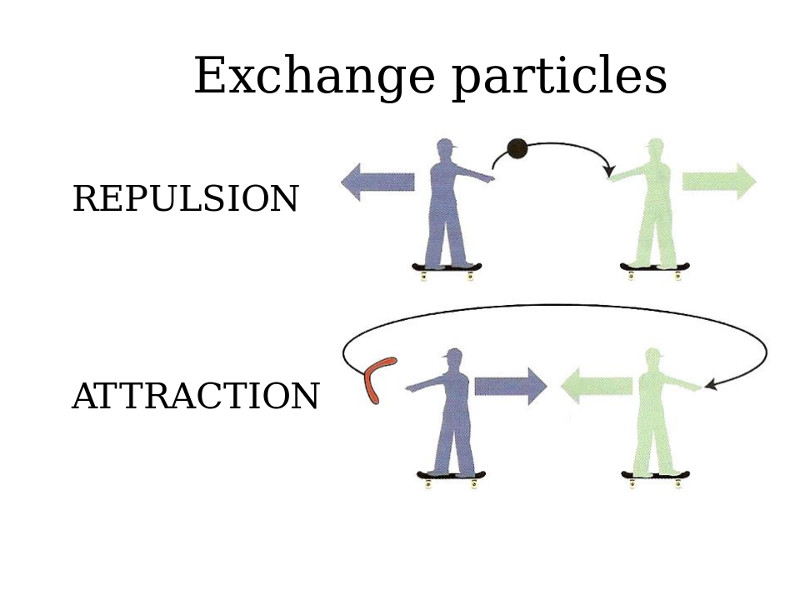
\includegraphics[width=7cm]{files/scambio_particelle.jpg}};
			\onslide<2->\node at (0,0) () {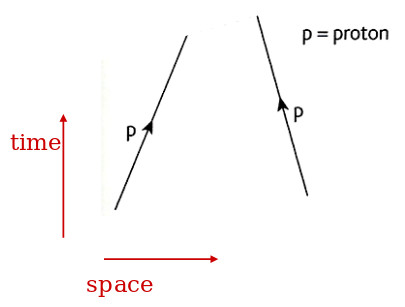
\includegraphics[width=5cm]{files/feynmanscuola01.jpg}};
			\onslide<3->\node at (5,0) () {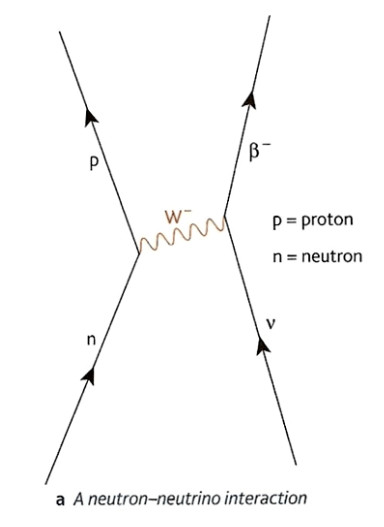
\includegraphics[width=4cm]{files/feynmanscuola02.jpg}};
		\end{tikzpicture}
	\end{center}
	\begin{itemize}
		\onslide<4>{\item \href{https://www.tes.com/teaching-resource/feynman-diagrams-6117223}{\textcolor{inaf}{Feynman diagrams - Teaching resources}}}
	\end{itemize}
\end{frame}
%
\begin{frame}[digressione]
	\frametitle{Digressione tecnica}
	\begin{block}{Principio di indeterminazione}
		\begin{displaymath}
			[p,q] = i \frac{h}{2\pi}
		\end{displaymath}
		\onslide<2->{
			\begin{displaymath}
				\Delta p \Delta q \geq \frac{h}{4\pi}
			\end{displaymath}}
	\end{block}
	\onslide<3->{
		\begin{block}{Particella virtuale \onslide<4->{$\rightarrow$ Scambio di numeri quantici}}
			Una particella che viola il principio di indeterminazione \onslide<4->{$\rightarrow$ Le particelle interagenti si scambiano i numeri quantici che, nel "mondo esterno" all'interazione costituiscono delle particelle}
		\end{block}}
\end{frame}
%
\begin{frame}[scuola02]
	\frametitle{Altre risorse quantistiche\footnote{via \href{http://pdg.lbl.gov/quarkdance/}{\textcolor{inaf}{Quark Dance}}}}
	\begin{itemize}
		\item \href{http://www.cpepphysics.org/Class_act.html}{\textcolor{inaf}{Attivit� dal Contemporary Physics Education Project}}
		\item \href{http://particleadventure.org/}{\textcolor{inaf}{Particle Adventure}}
		\begin{itemize}
			\item \href{https://play.google.com/store/apps/details?id=gov.lbl.physics}{\textcolor{inaf}{Applicazione per Android}}
		\end{itemize}
		\item \href{https://quarknet.org/}{\textcolor{inaf}{QuarkNet}}
	\end{itemize}
\end{frame}
\end{document}
